\documentclass[a4paper,12pt]{extarticle}
\usepackage[utf8x]{inputenc}
\usepackage[T1,T2A]{fontenc}
\usepackage[russian]{babel}
\usepackage{hyperref}
\usepackage{indentfirst}
\usepackage{listings}
\usepackage{color}
\usepackage{here}
\usepackage{array}
\usepackage{multirow}
\usepackage{graphicx}
\usepackage{amsmath}
\usepackage{amssymb}
\usepackage{makeidx}    

\usepackage{caption}
\renewcommand{\lstlistingname}{Программа} % заголовок листингов кода

\bibliographystyle{ugost2008ls}

\usepackage{listings}
\lstset{ %
extendedchars=\true,
keepspaces=true,
language=C,						% choose the language of the code
basicstyle=\footnotesize,		% the size of the fonts that are used for the code
numbers=left,					% where to put the line-numbers
numberstyle=\footnotesize,		% the size of the fonts that are used for the line-numbers
stepnumber=1,					% the step between two line-numbers. If it is 1 each line will be numbered
numbersep=5pt,					% how far the line-numbers are from the code
backgroundcolor=\color{white},	% choose the background color. You must add \usepackage{color}
showspaces=false				% show spaces adding particular underscores
showstringspaces=false,			% underline spaces within strings
showtabs=false,					% show tabs within strings adding particular underscores
frame=single,           		% adds a frame around the code
tabsize=2,						% sets default tabsize to 2 spaces
captionpos=t,					% sets the caption-position to top
breaklines=true,				% sets automatic line breaking
breakatwhitespace=false,		% sets if automatic breaks should only happen at whitespace
escapeinside={\%*}{*)},			% if you want to add a comment within your code
postbreak=\raisebox{0ex}[0ex][0ex]{\ensuremath{\color{red}\hookrightarrow\space}},
texcl=true,
inputpath=source,                     % директория с листингами
}

\usepackage[left=2cm,right=2cm,
top=2cm,bottom=2cm,bindingoffset=0cm]{geometry}

%% Нумерация картинок по секциям
\usepackage{chngcntr}
\counterwithin{figure}{section}
\counterwithin{table}{section}

%%Точки нумерации заголовков
\usepackage{titlesec}
\titlelabel{\thetitle.\quad}
\usepackage[dotinlabels]{titletoc}

%% Оформления подписи рисунка
\addto\captionsrussian{\renewcommand{\figurename}{Рисунок}}
\captionsetup[figure]{labelsep = period}

%% Подпись таблицы
\DeclareCaptionFormat{hfillstart}{\hfill#1#2#3\par}
\captionsetup[table]{format=hfillstart,labelsep=newline,justification=centering,skip=-10pt,textfont=bf}

%% Путь к каталогу с рисунками
\graphicspath{{pictures/}}


\begin{document}	% начало документа

% Титульная страница
\begin{titlepage}	% начало титульной страницы

	\begin{center}		% выравнивание по центру

		\large Санкт-Петербургский Политехнический Университет Петра Великого\\
		\large Институт компьютерных наук и технологий \\
		\large Кафедра компьютерных систем и программных технологий\\[6cm]
		% название института, затем отступ 6см
		
		\huge Телекоммуникационные технологии\\[0.5cm] % название работы, затем отступ 				%0,5см
		\large Отчет по лабораторной работе №3\\[0.1cm]
		\large Линейная фильтрация
		\\[5cm]

	\end{center}


	\begin{flushright} % выравнивание по правому краю
		\begin{minipage}{0.25\textwidth} % врезка в половину ширины текста
			\begin{flushleft} % выровнять её содержимое по левому краю

				\large\textbf{Работу выполнил:}\\
				\large Балсутьев В.А.\\
				\large {Группа:} 33501/4\\
				
				\large \textbf{Преподаватель:}\\
				\large Богач Н.В.

			\end{flushleft}
		\end{minipage}
	\end{flushright}
	
	\vfill % заполнить всё доступное ниже пространство

	\begin{center}
	\large Санкт-Петербург\\
	\large \the\year % вывести дату
	\end{center} % закончить выравнивание по центру

\thispagestyle{empty} % не нумеровать страницу
\end{titlepage} % конец титульной страницы

\vfill % заполнить всё доступное ниже пространство
	

% Содержание
% Содержание
\renewcommand\contentsname{\centerline{Содержание}}
\tableofcontents
\newpage


\section{Цель работы}
Изучение частотной и фазовой модуляции и демодуляции сигналов.
\section{Постановка задачи}
\begin{enumerate}
\item  сгенерировать однотональный сигнал низкой частоты 
\item  выполнить фазовую модуляцию и демодуляцию 
\item  выполнить частотную модуляцию и демодуляцию 
\item  получить спектр модулированного сигнала
\end{enumerate}

\section{Теоретическая информация}

\subsection{Модуляция}
Модуляция - это перенос спектра сигналов из низкочастотной области на заданную частоту. 
Это применяется для передачи сигнала в заданном частотном диапазоне.
Для модулирующего (исходного) сигнала $ S(t) $ в канале связи для передачи формируется  вспомогательный периодический высокочастотный сигнал $u(t)=f(t, [a_1,   a_2,   ...   a_m])$. Параметры $a_i$ определяют форму сигнала. 
При модуляции исходный сигнал $S(t)$ переносят на один из параметров $a_i$, форма сигнала $u(t)$ (несущей) изменяется и 
служит для переноса информации, содержащейся в сигнале $S(t)$. Обратная операция выделения сигнала $S(t)$ из 
модулированного сигнала $u(t)$ называется демодуляция.

\subsection{Однотональный сигнал}

Для генерации гармонического сигнала можно воспользоваться формулой\\ $signal = A*cos(2*\pi * f*t + \varphi)$,
 где $ A $ --- амплитуда сигнала, $f$ --- частота, $t$ --- вектор отсчетов времени, $\varphi$ --- смещение по фазе.

\subsection{Угловая модуляция}

При угловой модуляции в несущем гармоническом колебании $u(t) = U_m cos(\omega t + \varphi)$ 
значение амплитуды колебаний $U_m$ остается постоянным, а информация $s(t)$ переносится либо на частоту $\omega$, 
либо на фазовый угол $\varphi$. В обоих случаях текущее значение фазового угла гармонического 
колебания $u(t)$ определяет аргумент $\psi (t) = \omega t + \varphi$ ,
который называется полной фазой колебания.

\subsubsection{Фазовая модуляция}
При фазовой модуляции модулирующий сигнал определяет фазу несущего колебания
$\phi(t) = k s(t)$. Сигнал с фазовой модуляцией имеет вид 
\begin{equation}
    u(t) = U_m \cos(\omega_0 t + k s(t))
\end{equation}


\subsubsection{Частотная модуляция}
При частотной модуляции модулирующий сигнал определяет частоту несущего колебания.
Сигнал с частотной модуляцией имеет вид  
\begin{equation}
	u(t) = U_m cos(\omega_0 t + k \int_{0}^{t} s(t) dt)
\end{equation}

\section{Ход выполнения работы}

\subsection{Однотональный сигнал}
Получим обычный гармонический сигнал  $s(t) = Acos(2 \pi ft + \phi)$ 
\begin{figure}[H]
	\begin{center}
		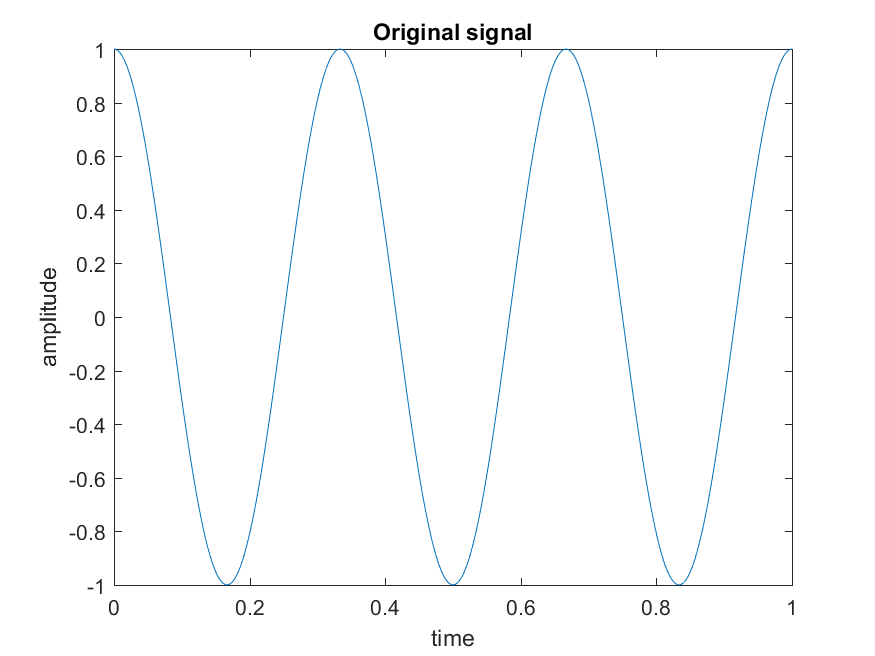
\includegraphics[scale=0.7]{003_origin_sig.png}
		\caption{Однотональный сигнал} 
		\label{pic:001} % название для ссылок внутри кода
	\end{center}
\end{figure}
Построим его спектр:
\begin{figure}[H]
	\begin{center}
		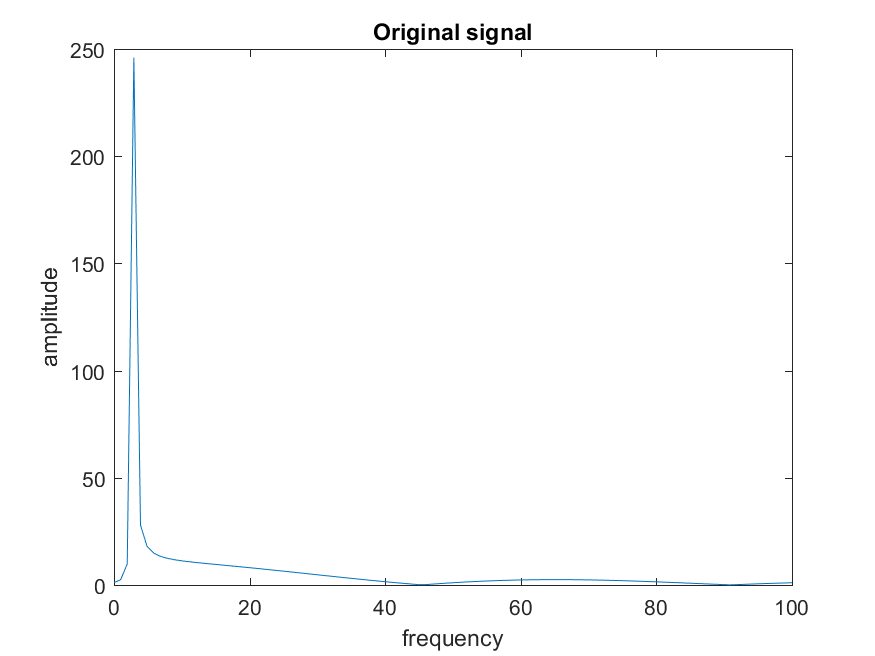
\includegraphics[scale=0.7]{001_origin_spec.png}
		\caption{Однотональный сигнал} 
		\label{pic:002} % название для ссылок внутри кода
	\end{center}
\end{figure}

\subsection{Фазовая модуляция}
Промодулируем и также получим спектр:
\begin{figure}[H]
	\begin{center}
		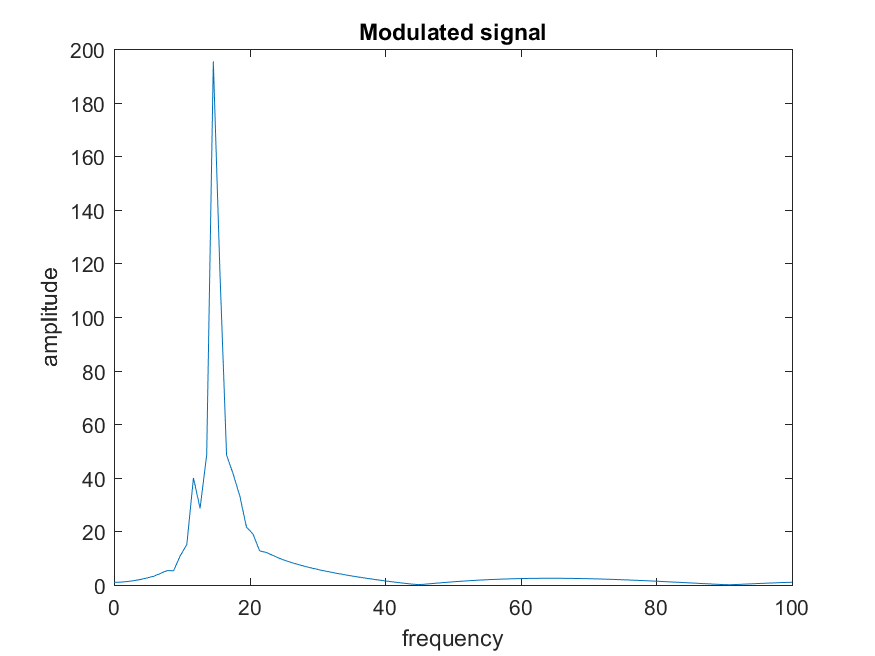
\includegraphics[scale=0.7]{002_mod_spec.png}
		\caption{Спектр модулированного сигнала} 
		\label{pic:003} % название для ссылок внутри кода
	\end{center}
\end{figure}
Проведем демодуляцию и посмотрим результаты:
\begin{figure}[H]
	\begin{center}
		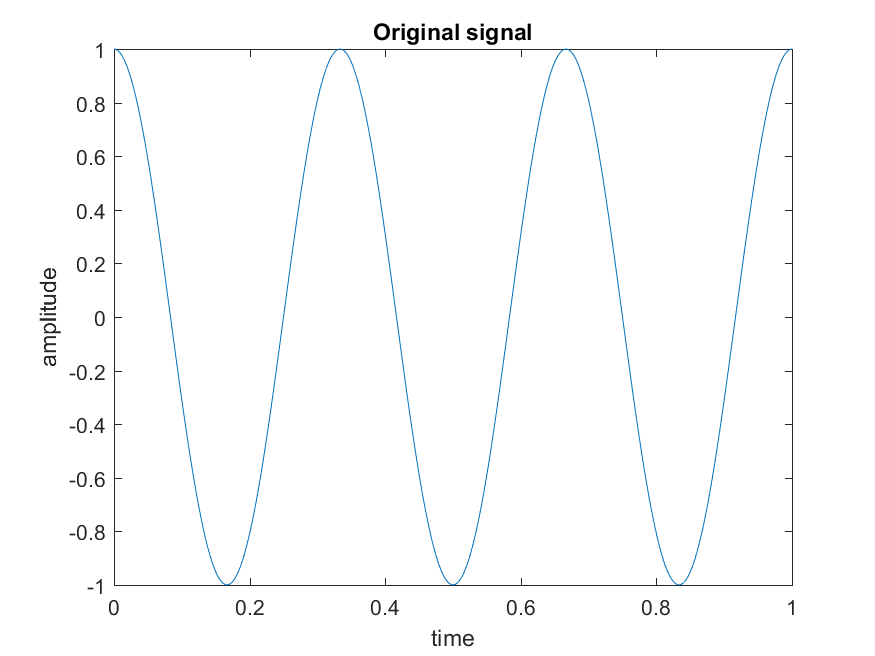
\includegraphics[scale=0.7]{004_recovered.png}
		\caption{Демодулированный сигнал(фазовая модуляция)} 
		\label{pic:004} % название для ссылок внутри кода
	\end{center}
\end{figure}
Cпектр:
\begin{figure}[H]
	\begin{center}
		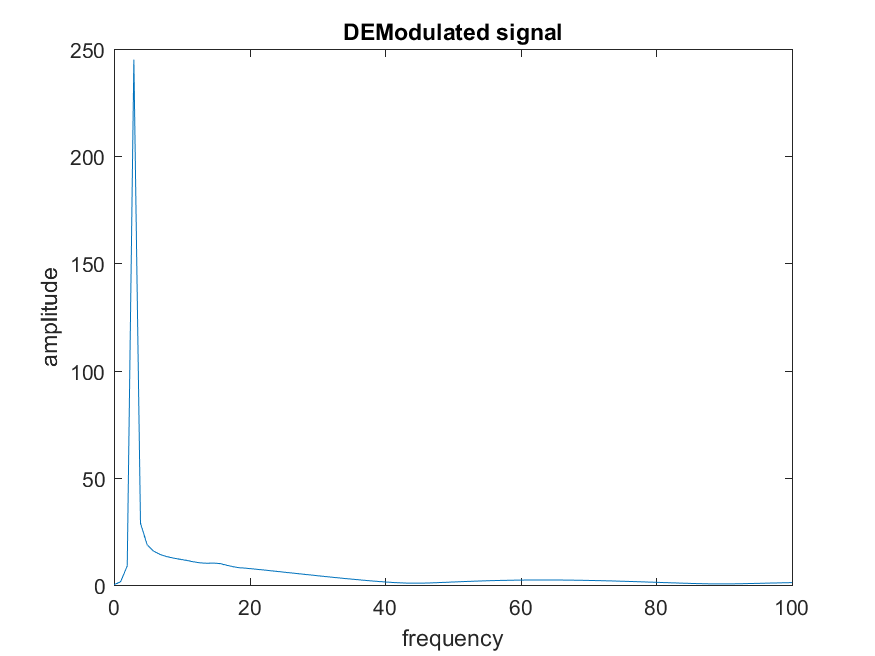
\includegraphics[scale=0.7]{005_demod_spec.png}
		\caption{Спектр демодулированного сигнала(фазовая демодуляция)} 
		\label{pic:005} % название для ссылок внутри кода
	\end{center}
\end{figure} 
Очевидно, что исходный сигнал совпадает с демодулированным, получившийся спектр также это подтверждает.   

\subsection{Частотная модуляция}
Промодулировав частотно наш сигнал, получили следующий график:
\begin{figure}[H]
	\begin{center}
		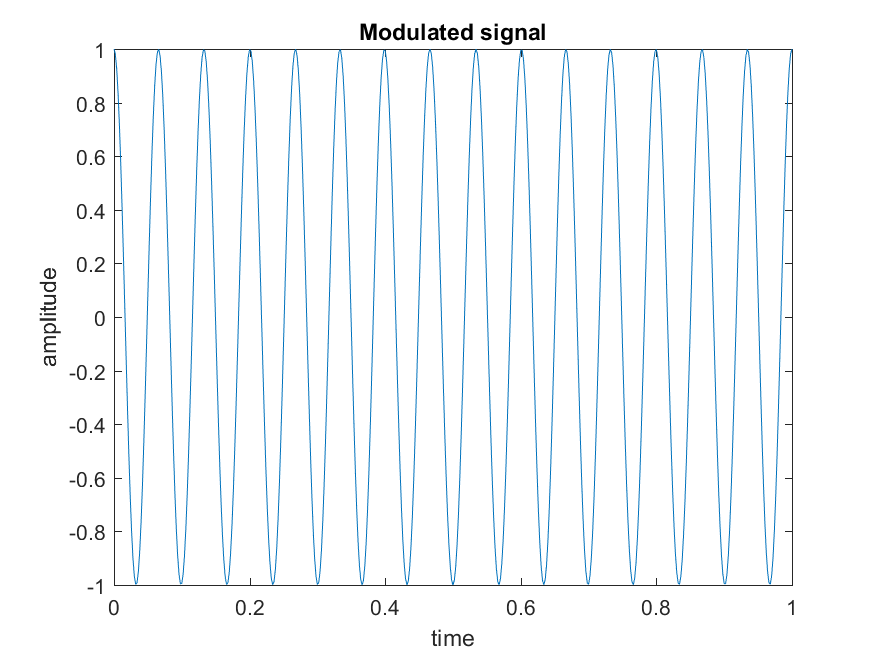
\includegraphics[scale=0.7]{006_mod_sig.png}
		\caption{Модулированного сигнала(частотная модуляция)} 
		\label{pic:006} % название для ссылок внутри кода
	\end{center}
\end{figure} 
Далее получили демодулированный сигнал, для которого вычислили преобразование Фурье и постороили амплитудный спектр.
\begin{figure}[H]
	\begin{center}
		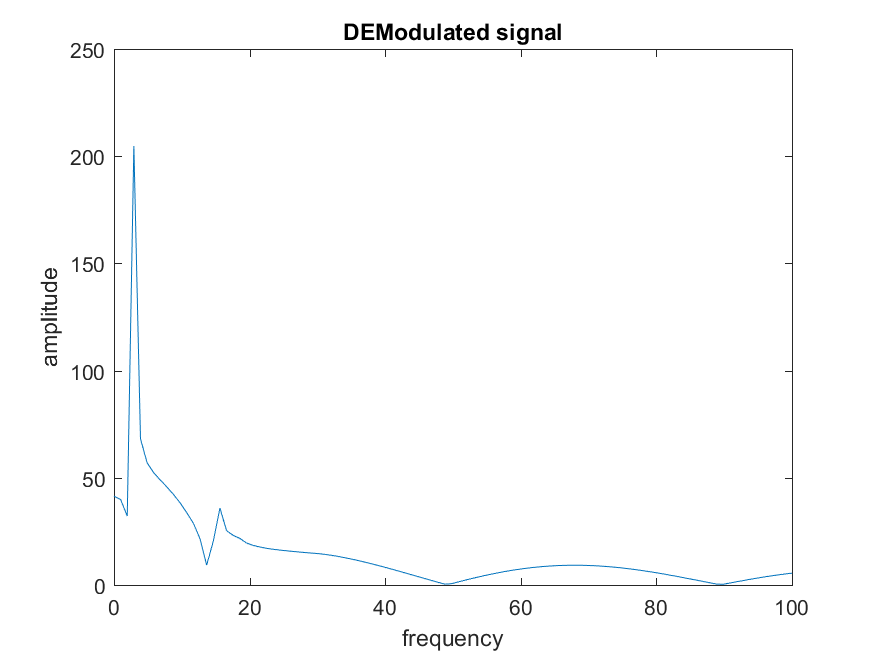
\includegraphics[scale=0.7]{007_demod_spec.png}
		\caption{Спектр демодулированного сигнала(частотная модуляция)} 
		\label{pic:007} % название для ссылок внутри кода
	\end{center}
\end{figure} 

Как и в случае с фазовой модуляцией-демодуляцией исходный сигнал демодулирован хорошо.
Код всей лабораторной работы на Matlab приведен ниже.

\lstinputlisting[
	label=code:lab05,
	caption={lab05.m},% для печати символ '_' требует выходной символ '\'
]{lab05.m}
\parindent=1cm % командна \lstinputlisting сбивает параментры отступа

\section{Выводы}
Таким образом нам удалось на качественном уровне понять основы угловой модуляции и выполнить модулирование совместно с демодулированием однотоннального сигнала. Экспериментально удалось подтвердить, что данные типы модуляции на хорошем уровне позволяют передавать сигнал. Также следует отметить, что фазовая модуляция совместно с частотной модуляцией в связи с высоким КПД и другими свойствами достаточно часто используются в Радиолокации. А значит полученные нами знания в результате выполнения данной работы пригодятся в самом обозримом будующем - на военной кафедре:).   
\end{document}
